% Asset ID: AS2MeasuresLocationSpreadTikZ-006
% Purpose: Show how y = ax + b affects mean, standard deviation and variance.
% Boundary note: Coding is included as enrichment/support, not as a standalone supplied CCEA LO.
\documentclass[tikz,border=8pt]{standalone}
\usepackage{amsmath}
\usetikzlibrary{positioning, arrows.meta}
\begin{document}
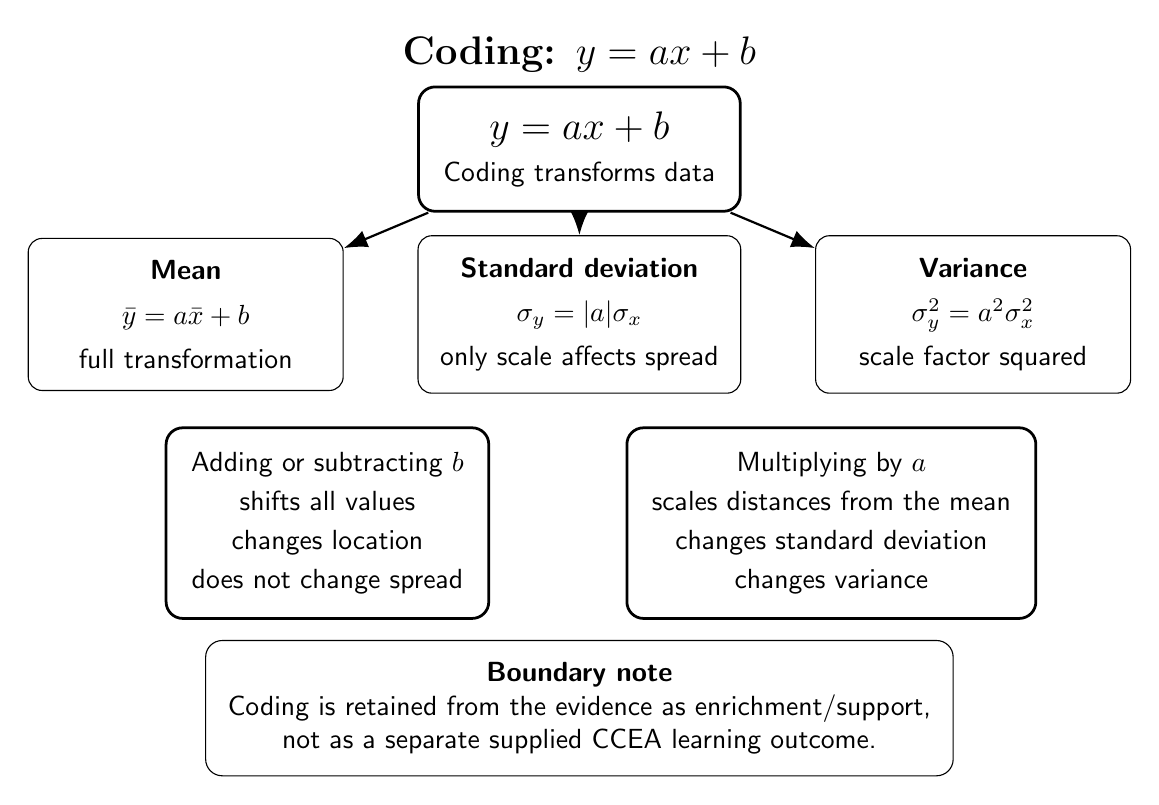
\begin{tikzpicture}[font=\sffamily, main/.style={draw, rounded corners=6pt, align=center, inner sep=9pt, line width=1pt}, result/.style={draw, rounded corners=5pt, align=center, inner sep=8pt, minimum width=4cm}, arrow/.style={-{Latex[length=3mm]}, thick}]
\node[font=\Large\bfseries] at (0,4.5) {Coding: $y=ax+b$};
\node[main] (code) at (0,3.3) {\Large $y=ax+b$\\[3pt]Coding transforms data};
\node[result] (mean) at (-5,1.2) {\bfseries Mean\\[4pt]$\bar{y}=a\bar{x}+b$\\[4pt]full transformation};
\node[result] (sd) at (0,1.2) {\bfseries Standard deviation\\[4pt]$\sigma_y=|a|\sigma_x$\\[4pt]only scale affects spread};
\node[result] (var) at (5,1.2) {\bfseries Variance\\[4pt]$\sigma_y^2=a^2\sigma_x^2$\\[4pt]scale factor squared};
\draw[arrow] (code) -- (mean);\draw[arrow] (code) -- (sd);\draw[arrow] (code) -- (var);
\node[main] at (-3.2,-1.45) {Adding or subtracting $b$\\[2pt]shifts all values\\[2pt]changes location\\[2pt]does not change spread};
\node[main] at (3.2,-1.45) {Multiplying by $a$\\[2pt]scales distances from the mean\\[2pt]changes standard deviation\\[2pt]changes variance};
\node[draw, rounded corners=6pt, align=center, inner sep=8pt] at (0,-3.8) {\bfseries Boundary note\\Coding is retained from the evidence as enrichment/support,\\not as a separate supplied CCEA learning outcome.};
\end{tikzpicture}
\end{document}
